% Options for packages loaded elsewhere
\PassOptionsToPackage{unicode}{hyperref}
\PassOptionsToPackage{hyphens}{url}
%
\documentclass[
]{article}
\usepackage{amsmath,amssymb}
\usepackage{iftex}
\ifPDFTeX
  \usepackage[T1]{fontenc}
  \usepackage[utf8]{inputenc}
  \usepackage{textcomp} % provide euro and other symbols
\else % if luatex or xetex
  \usepackage{unicode-math} % this also loads fontspec
  \defaultfontfeatures{Scale=MatchLowercase}
  \defaultfontfeatures[\rmfamily]{Ligatures=TeX,Scale=1}
\fi
\usepackage{lmodern}
\ifPDFTeX\else
  % xetex/luatex font selection
\fi
% Use upquote if available, for straight quotes in verbatim environments
\IfFileExists{upquote.sty}{\usepackage{upquote}}{}
\IfFileExists{microtype.sty}{% use microtype if available
  \usepackage[]{microtype}
  \UseMicrotypeSet[protrusion]{basicmath} % disable protrusion for tt fonts
}{}
\makeatletter
\@ifundefined{KOMAClassName}{% if non-KOMA class
  \IfFileExists{parskip.sty}{%
    \usepackage{parskip}
  }{% else
    \setlength{\parindent}{0pt}
    \setlength{\parskip}{6pt plus 2pt minus 1pt}}
}{% if KOMA class
  \KOMAoptions{parskip=half}}
\makeatother
\usepackage{xcolor}
\usepackage[margin=1in]{geometry}
\usepackage{longtable,booktabs,array}
\usepackage{calc} % for calculating minipage widths
% Correct order of tables after \paragraph or \subparagraph
\usepackage{etoolbox}
\makeatletter
\patchcmd\longtable{\par}{\if@noskipsec\mbox{}\fi\par}{}{}
\makeatother
% Allow footnotes in longtable head/foot
\IfFileExists{footnotehyper.sty}{\usepackage{footnotehyper}}{\usepackage{footnote}}
\makesavenoteenv{longtable}
\usepackage{graphicx}
\makeatletter
\def\maxwidth{\ifdim\Gin@nat@width>\linewidth\linewidth\else\Gin@nat@width\fi}
\def\maxheight{\ifdim\Gin@nat@height>\textheight\textheight\else\Gin@nat@height\fi}
\makeatother
% Scale images if necessary, so that they will not overflow the page
% margins by default, and it is still possible to overwrite the defaults
% using explicit options in \includegraphics[width, height, ...]{}
\setkeys{Gin}{width=\maxwidth,height=\maxheight,keepaspectratio}
% Set default figure placement to htbp
\makeatletter
\def\fps@figure{htbp}
\makeatother
\setlength{\emergencystretch}{3em} % prevent overfull lines
\providecommand{\tightlist}{%
  \setlength{\itemsep}{0pt}\setlength{\parskip}{0pt}}
\setcounter{secnumdepth}{5}
\newlength{\cslhangindent}
\setlength{\cslhangindent}{1.5em}
\newlength{\csllabelwidth}
\setlength{\csllabelwidth}{3em}
\newlength{\cslentryspacingunit} % times entry-spacing
\setlength{\cslentryspacingunit}{\parskip}
\newenvironment{CSLReferences}[2] % #1 hanging-ident, #2 entry spacing
 {% don't indent paragraphs
  \setlength{\parindent}{0pt}
  % turn on hanging indent if param 1 is 1
  \ifodd #1
  \let\oldpar\par
  \def\par{\hangindent=\cslhangindent\oldpar}
  \fi
  % set entry spacing
  \setlength{\parskip}{#2\cslentryspacingunit}
 }%
 {}
\usepackage{calc}
\newcommand{\CSLBlock}[1]{#1\hfill\break}
\newcommand{\CSLLeftMargin}[1]{\parbox[t]{\csllabelwidth}{#1}}
\newcommand{\CSLRightInline}[1]{\parbox[t]{\linewidth - \csllabelwidth}{#1}\break}
\newcommand{\CSLIndent}[1]{\hspace{\cslhangindent}#1}
\ifLuaTeX
  \usepackage{selnolig}  % disable illegal ligatures
\fi
\IfFileExists{bookmark.sty}{\usepackage{bookmark}}{\usepackage{hyperref}}
\IfFileExists{xurl.sty}{\usepackage{xurl}}{} % add URL line breaks if available
\urlstyle{same}
\hypersetup{
  pdftitle={Lessons learned: creating tutorials teaching Agent-Based Modelling for Archaeologists},
  hidelinks,
  pdfcreator={LaTeX via pandoc}}

\title{Lessons learned: creating tutorials teaching Agent-Based Modelling for Archaeologists}
\author{true \and true \and true \and true \and true \and true \and true \and true \and true}
\date{}

\begin{document}
\maketitle

{
\setcounter{tocdepth}{2}
\tableofcontents
}
\hypertarget{introduction}{%
\section{Introduction}\label{introduction}}

ABM application increased in Archaeology

Other teaching material available SPOC (Scherjon, Romanowska and Lambers 2019)

New handbook (Romanowska, Wren and Crabtree 2021)

No formal training

EU project \url{https://erasmus-plus.ec.europa.eu/nl/projects/search/details/2021-2-IE01-KA220-VET-000049054}

\hypertarget{method}{%
\section{Method}\label{method}}

During the project we have developed tutorials. The tutorials were first designed using storyboards which were later converted into tutorials using NetLOGO Web (\url{https://www.netlogoweb.org/launch}) and Javascript (). The tutorials were developed together and we worked together using GitHub (\url{https://github.com/lljvdk/EU-ABMA/}). During the project initial testing was done with all authors and issues in GitHub were used to tackle bugs.

The tutorial were tested during various online and in-person conferences. The in-person conferences were attended by several people from the project team. During the online events we were always present with several people and enabled participants to go to break-out rooms if they needed any help or wanted to discuss things. In addition, we also had students working with the tutorials at Saxion University of applied sciences and Leiden University. We used the feedback of the participants to improve the tutorials. The feedback was obtained structurally using two surveys using Qualtrics. The participants of the events were asked to answer questions of a survey before participating. We used the answers to understand what the background of the participants was and to get an estimate of their level of knowledge in relation to ABM (see appendix \ldots{} for the questions). After the participants worked with the tutorials during the event they were asked to answer a second survey. Questions of this survey were aimed at the measuring the effectiveness of the tutorials and getting feedback on the workshop and tutorials (see appendix \ldots{} for the questions). For some events participants had to register beforehand and we were able to send the pre-workshop survey by email. At other events no registration was possible or necessary and the pre-workshop survey was given at the start of the event. The post-workshop survey was distributed using QR-codes or links at the end of the workshop during the event. After each event we have improved the tutorials based on the received feedback.

\begin{longtable}[]{@{}
  >{\raggedright\arraybackslash}p{(\columnwidth - 8\tabcolsep) * \real{0.2000}}
  >{\raggedright\arraybackslash}p{(\columnwidth - 8\tabcolsep) * \real{0.2000}}
  >{\raggedright\arraybackslash}p{(\columnwidth - 8\tabcolsep) * \real{0.2000}}
  >{\raggedright\arraybackslash}p{(\columnwidth - 8\tabcolsep) * \real{0.2000}}
  >{\raggedright\arraybackslash}p{(\columnwidth - 8\tabcolsep) * \real{0.2000}}@{}}
\caption{Conferences, events and situations were the workshops given and the tutorials were tested.}\tabularnewline
\toprule\noalign{}
\begin{minipage}[b]{\linewidth}\raggedright
Conference or event
\end{minipage} & \begin{minipage}[b]{\linewidth}\raggedright
Period
\end{minipage} & \begin{minipage}[b]{\linewidth}\raggedright
Online, in person or hybrid
\end{minipage} & \begin{minipage}[b]{\linewidth}\raggedright
Number of participants
\end{minipage} & \begin{minipage}[b]{\linewidth}\raggedright
Number of registrations
\end{minipage} \\
\midrule\noalign{}
\endfirsthead
\toprule\noalign{}
\begin{minipage}[b]{\linewidth}\raggedright
Conference or event
\end{minipage} & \begin{minipage}[b]{\linewidth}\raggedright
Period
\end{minipage} & \begin{minipage}[b]{\linewidth}\raggedright
Online, in person or hybrid
\end{minipage} & \begin{minipage}[b]{\linewidth}\raggedright
Number of participants
\end{minipage} & \begin{minipage}[b]{\linewidth}\raggedright
Number of registrations
\end{minipage} \\
\midrule\noalign{}
\endhead
\bottomrule\noalign{}
\endlastfoot
CAA Amsterdam & April 2023 & In person & 36 & 53 \\
EAA Belfast & August 2023 & In person & 21 & No registration \\
CAA-DE/NL-Fl Online workshop & October 2023 & Online & 40 & 76 \\
Reuvensdagen & November 2023 & In person & 13 & No registration \\
CAA-UK & November 2023 & Hybrid & 53 & \\
Leiden (course) & December 2023 & In person & 11 & No registration \\
Aarhus & January/February 2024 & Online & 176 & \textgreater500 \\
Saxion & March 2023-January 2024 & In person & 18 & No registration \\
\textbf{Total} & & & \textbf{368} & \textbf{\textgreater628} \\
\end{longtable}

The surveys were analysed using R (R Core Team 2023). The following packages were used for analyses: ggplot2 (Wickham 2016), dplyr (Wickham et al. 2023), tidyr (Wickham, Vaughan and Girlich 2023), forcats(Wickham 2023a), lubridate (Grolemund and Wickham 2011) and stringr (Wickham 2023b). The date and the code is available at \url{https://github.com/RonaldVisser/ABM_tutorials} and (\ldots{} insert Zenodo reference\ldots)

Over the course of the project three groups of students worked on the project during the Smart Solutions Semester at Saxion University of Applied Sciences. This is an interdisciplinary semester in which students of at least three different study-programmes or disciplines work together on a complex problem/project (\url{https://www.saxion.edu/business-and-research/collaborate-with-saxion/smart-solutions}). The backgrounds of the various students were diverse: Applied Computer Science, Archaeology, Business Management Studies, Creative Business, Creative Media \& Game Technologies, and ICT. The diverse groups of students contributed with new ideas, developing educational material, testing the tutorials and developing a style for the website and other materials.

\hypertarget{results}{%
\section{Results}\label{results}}

\hypertarget{workhops-and-tutorials}{%
\subsection{Workhops and tutorials}\label{workhops-and-tutorials}}

\hypertarget{before-the-workhops}{%
\subsection{Before the workhops}\label{before-the-workhops}}

A large proportion of the participants of the workshops gave us information using the survey before the workshops (172 of 368 participants). The respondents came from many different countries all over the world (see Figure \ref{fig:nationality}. The number of female respondents slightly outnumber the male ones and a small group did not share their gender and two were non-binary (see Figure \ref{fig:gender-age}). The ages of the respondents ranged from below 20 to over 70, reaching people in different age classes, although the majority was aged between 20 and 40. It seems that the different events also had a slightly different distribution of both gender and age. For example, more older people attended the workshop at the CAA conference in April 2023 and more male people were present during the workshop at the Reuvensdagen in November 2023.

\begin{figure}
\centering
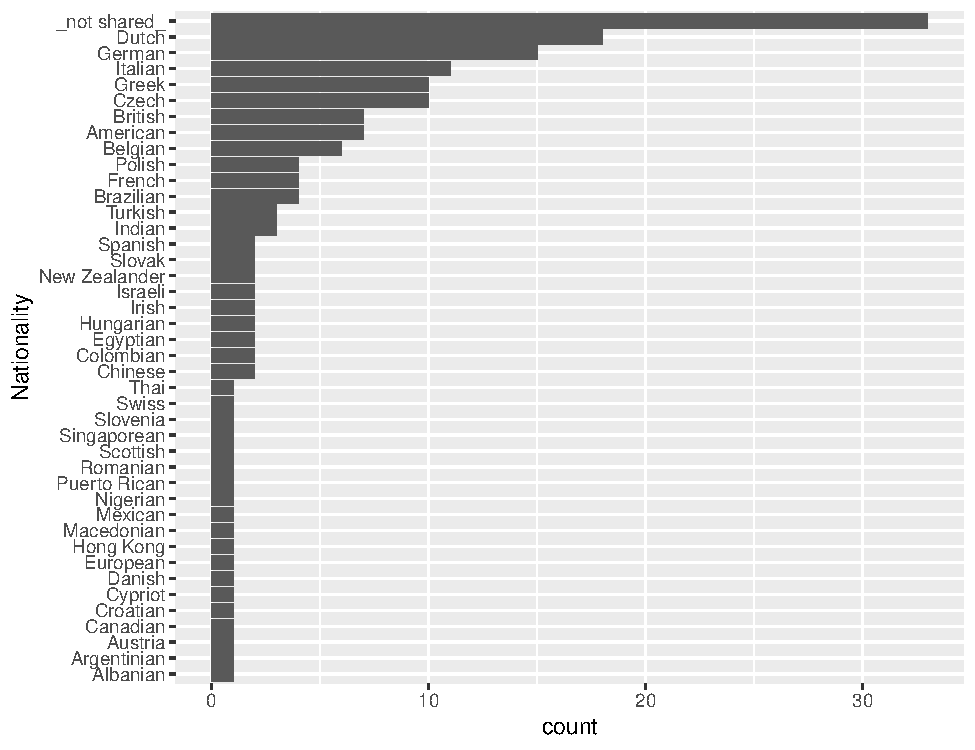
\includegraphics{paper_files/figure-latex/nationality-1.pdf}
\caption{\label{fig:nationality}The nationality of the participants that filled in the survey.}
\end{figure}

\begin{figure}
\centering
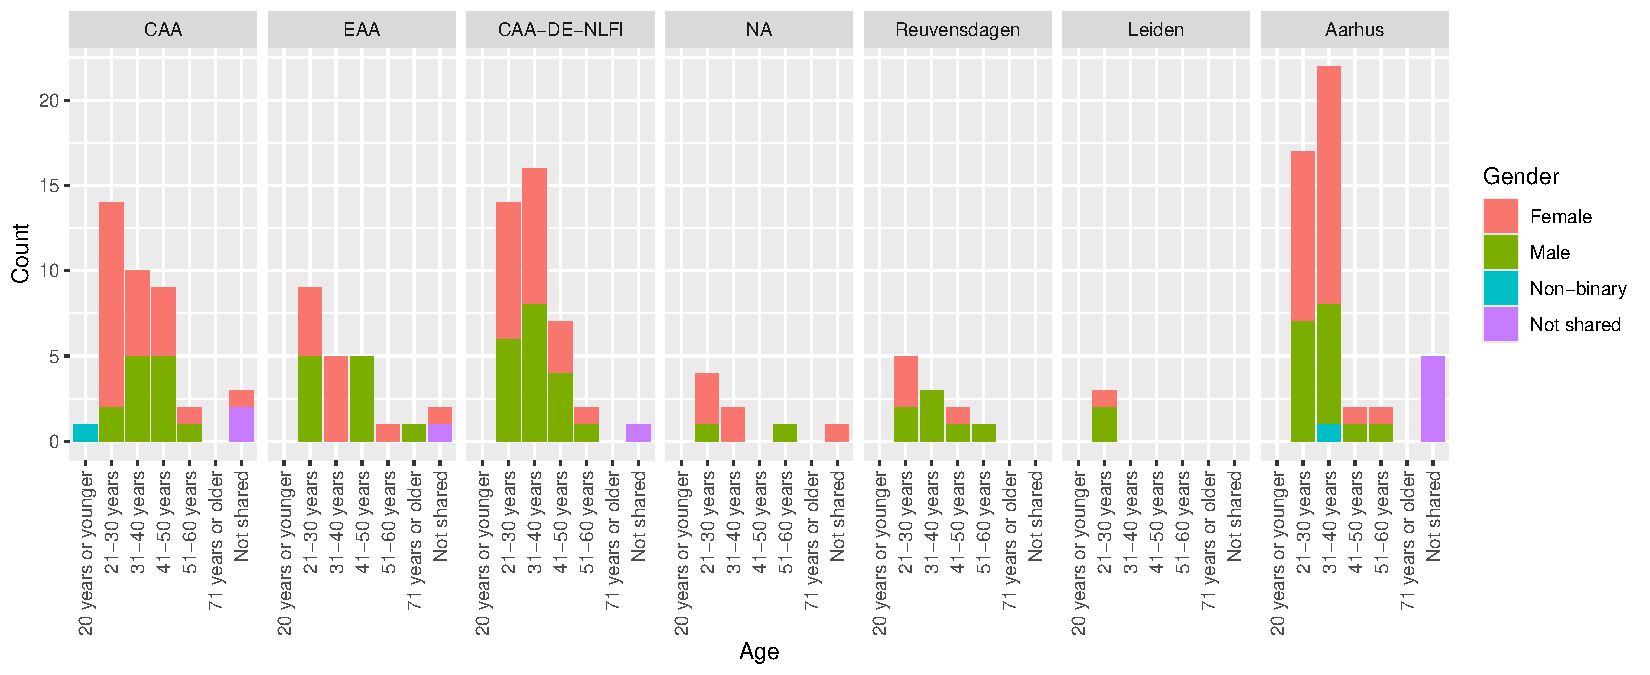
\includegraphics{paper_files/figure-latex/gender-age-1.pdf}
\caption{\label{fig:gender-age}The gender and age of the respondents for each workshop}
\end{figure}

Most of the respondents had several skills with computer applications in archaeology (see Figure \ref{fig:computer-skills}), and many of them did have some knowledge of ABM, although a large group was completely new to the subject. The majority had never applied ABM before participating in the workshops with 14 having applied ABM. It is interesting to note that many respondents did know what kind of software was available for ABM (see Figure \ref{fig:abm-knowledge}).

\begin{figure}
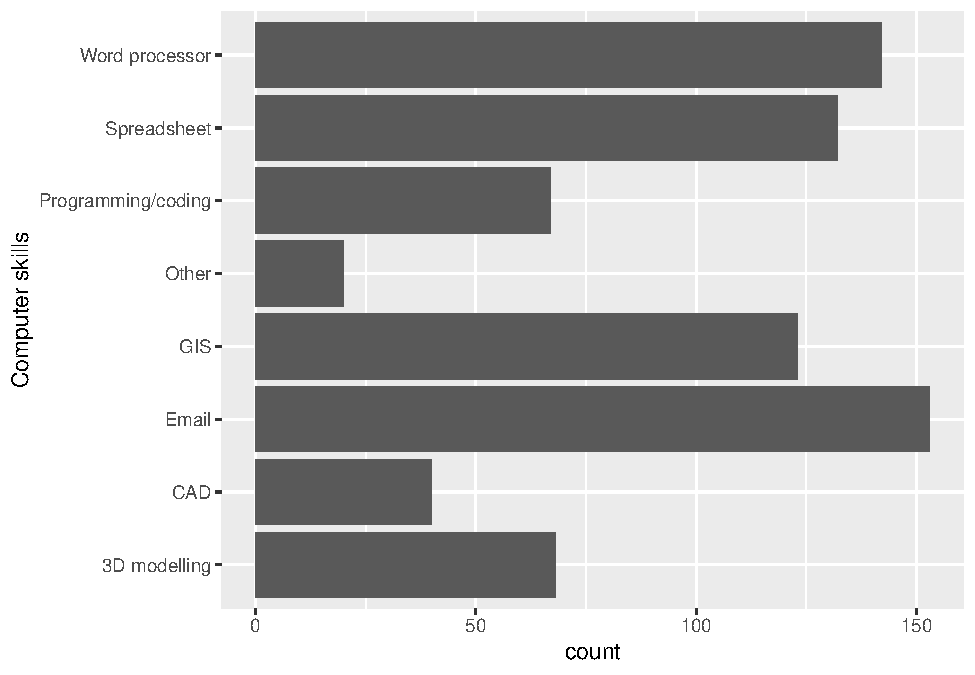
\includegraphics[width=0.5\linewidth]{paper_files/figure-latex/computer-skills-1} \caption{The computer skills of the respondents.}\label{fig:computer-skills}
\end{figure}

\begin{figure}
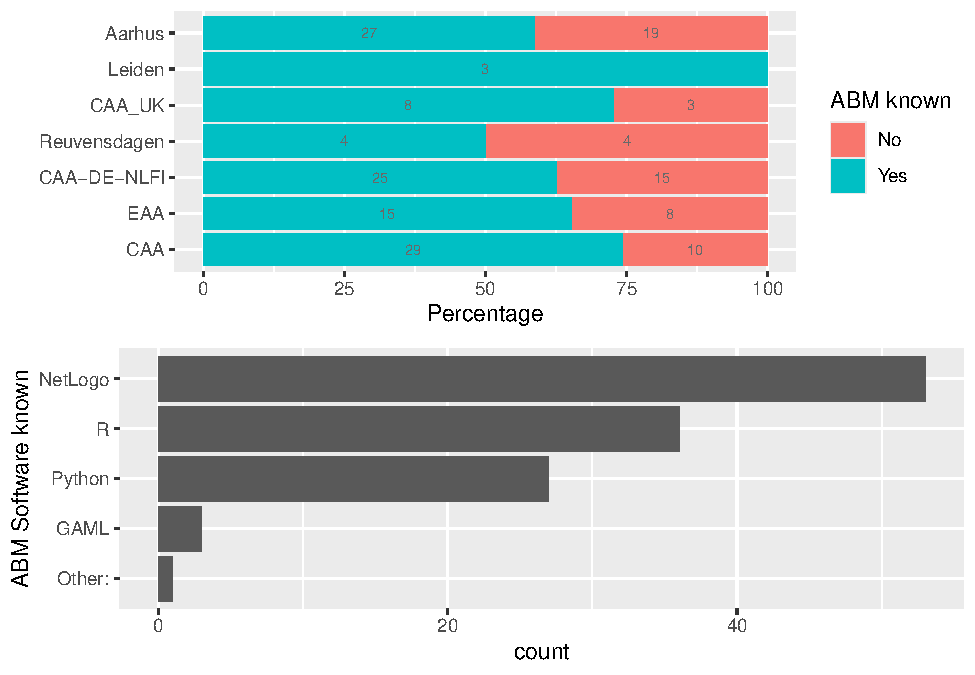
\includegraphics[width=0.5\linewidth]{paper_files/figure-latex/abm-knowledge-1} 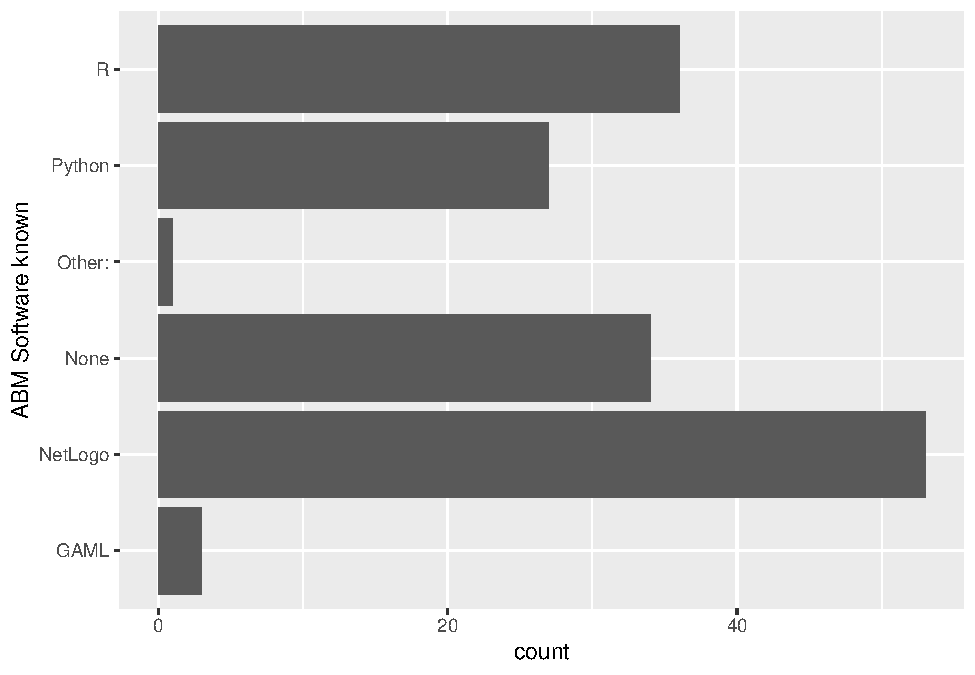
\includegraphics[width=0.5\linewidth]{paper_files/figure-latex/abm-knowledge-2} \caption{Respondents knowledge and experience with ABM.}\label{fig:abm-knowledge}
\end{figure}

As shown above, the respondents had some knowledge on ABM in general, but did not know how to apply this or had never applied this before. The respondents were also asked how they rated the available knowledge on ABM (Figure \ref{fig:available-theory}). While the largest group of them had no opinion on the subject, a very large proportion of the responded answered that they rated the available theory on ABM as limited and a smaller group as sufficient. A minority rated the available theory on ABM as more than sufficient. This clearly shows the need for better educational material.

\begin{figure}
\centering
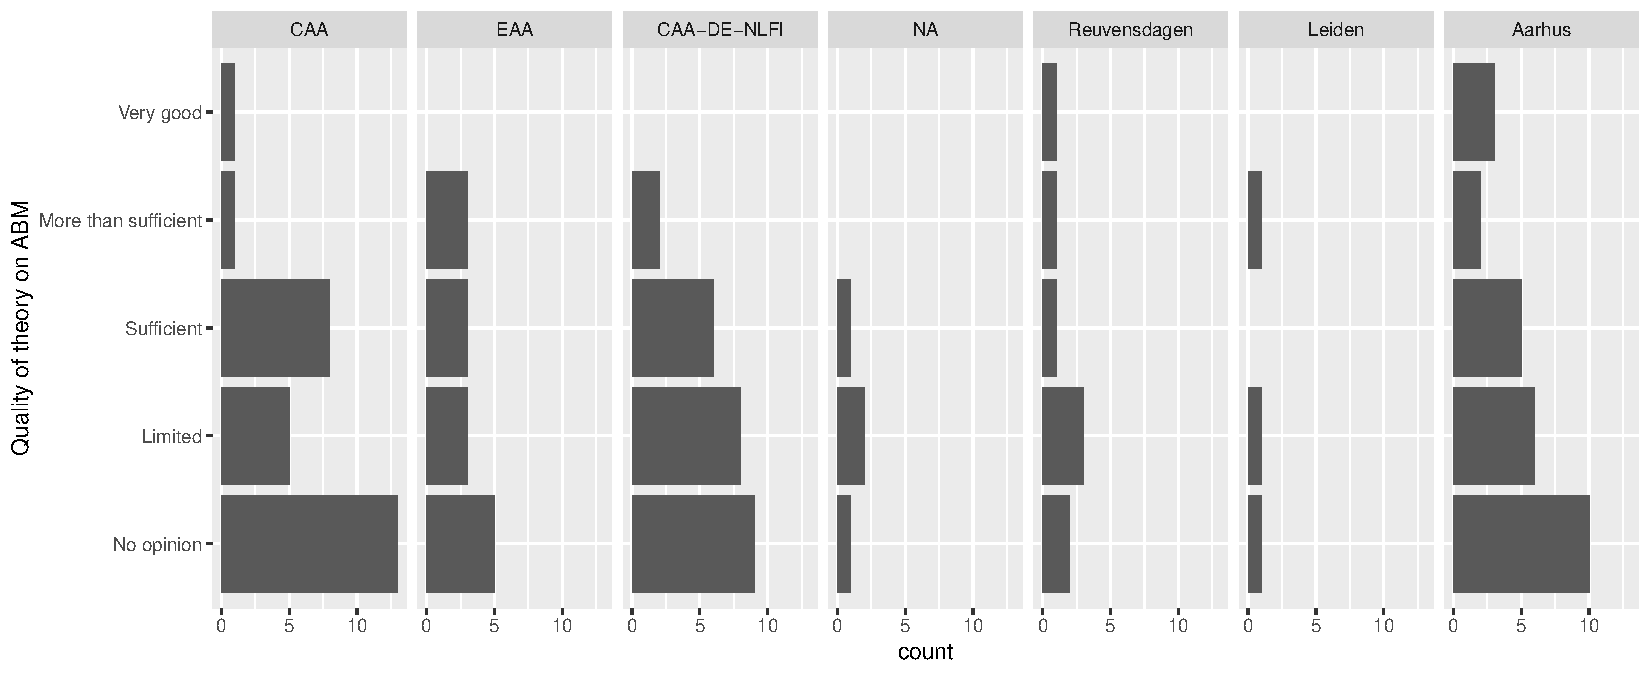
\includegraphics{paper_files/figure-latex/available-theory-1.pdf}
\caption{\label{fig:available-theory}Respondents optionion on the quality of theory on ABM faceted out by event.}
\end{figure}

\hypertarget{after-tutorial}{%
\subsection{After tutorial}\label{after-tutorial}}

A large proportion of the participants of the workshops gave us information using the survey after the workshops (171 of 368 participants), a similar proportion as those responding to the survey before the workshop.

The respondents

\begin{figure}
\centering
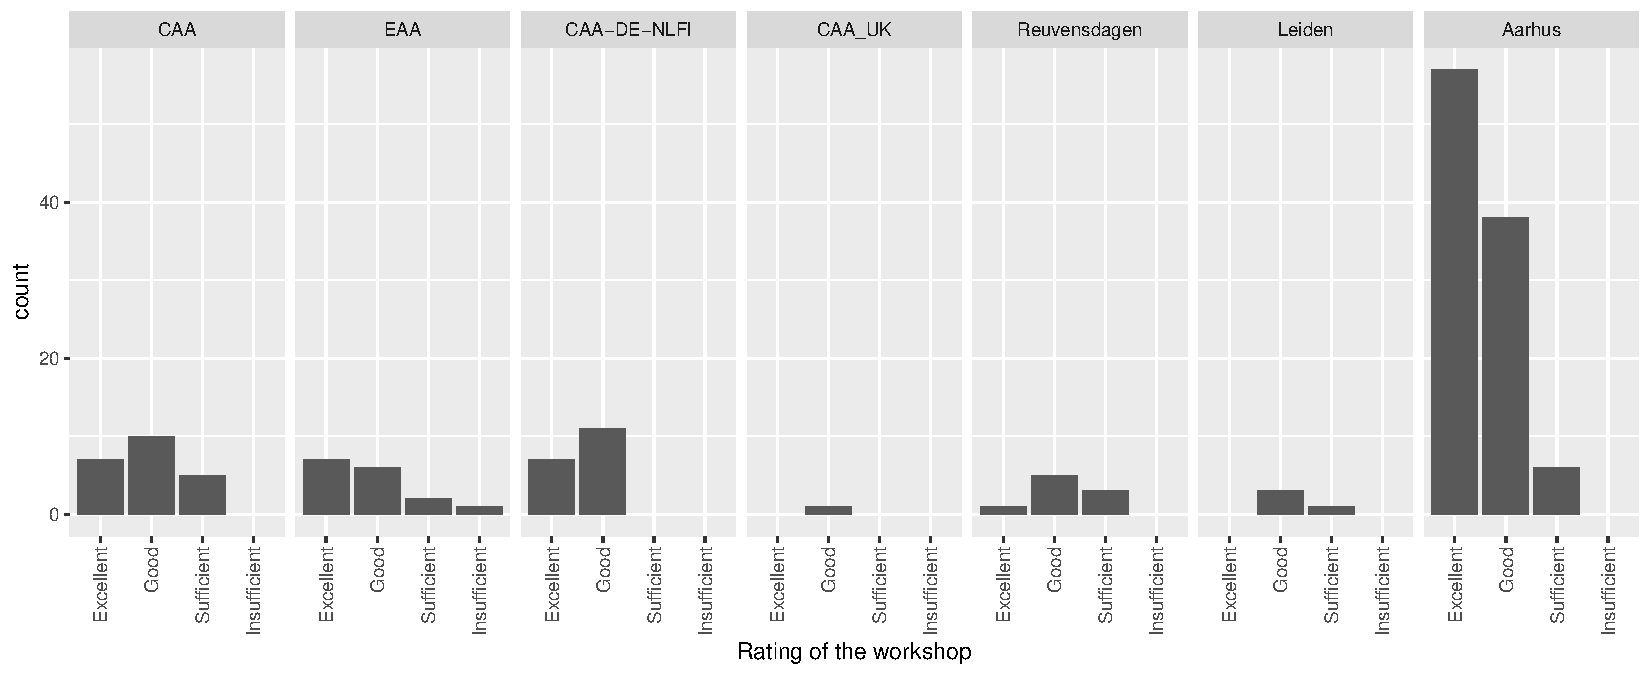
\includegraphics{paper_files/figure-latex/rating-workshop-1.pdf}
\caption{\label{fig:rating-workshop}Respondents rating of the workshop in general faceted for each event.}
\end{figure}

The majority of the respondents were enthusiastic about the teaching material, with the majority rating it as excellent or good. The teachers were even rated better than the teaching material, with more respondents rating them as excellent (see Figure \ref{fig:rating-teaching}).

\begin{figure}
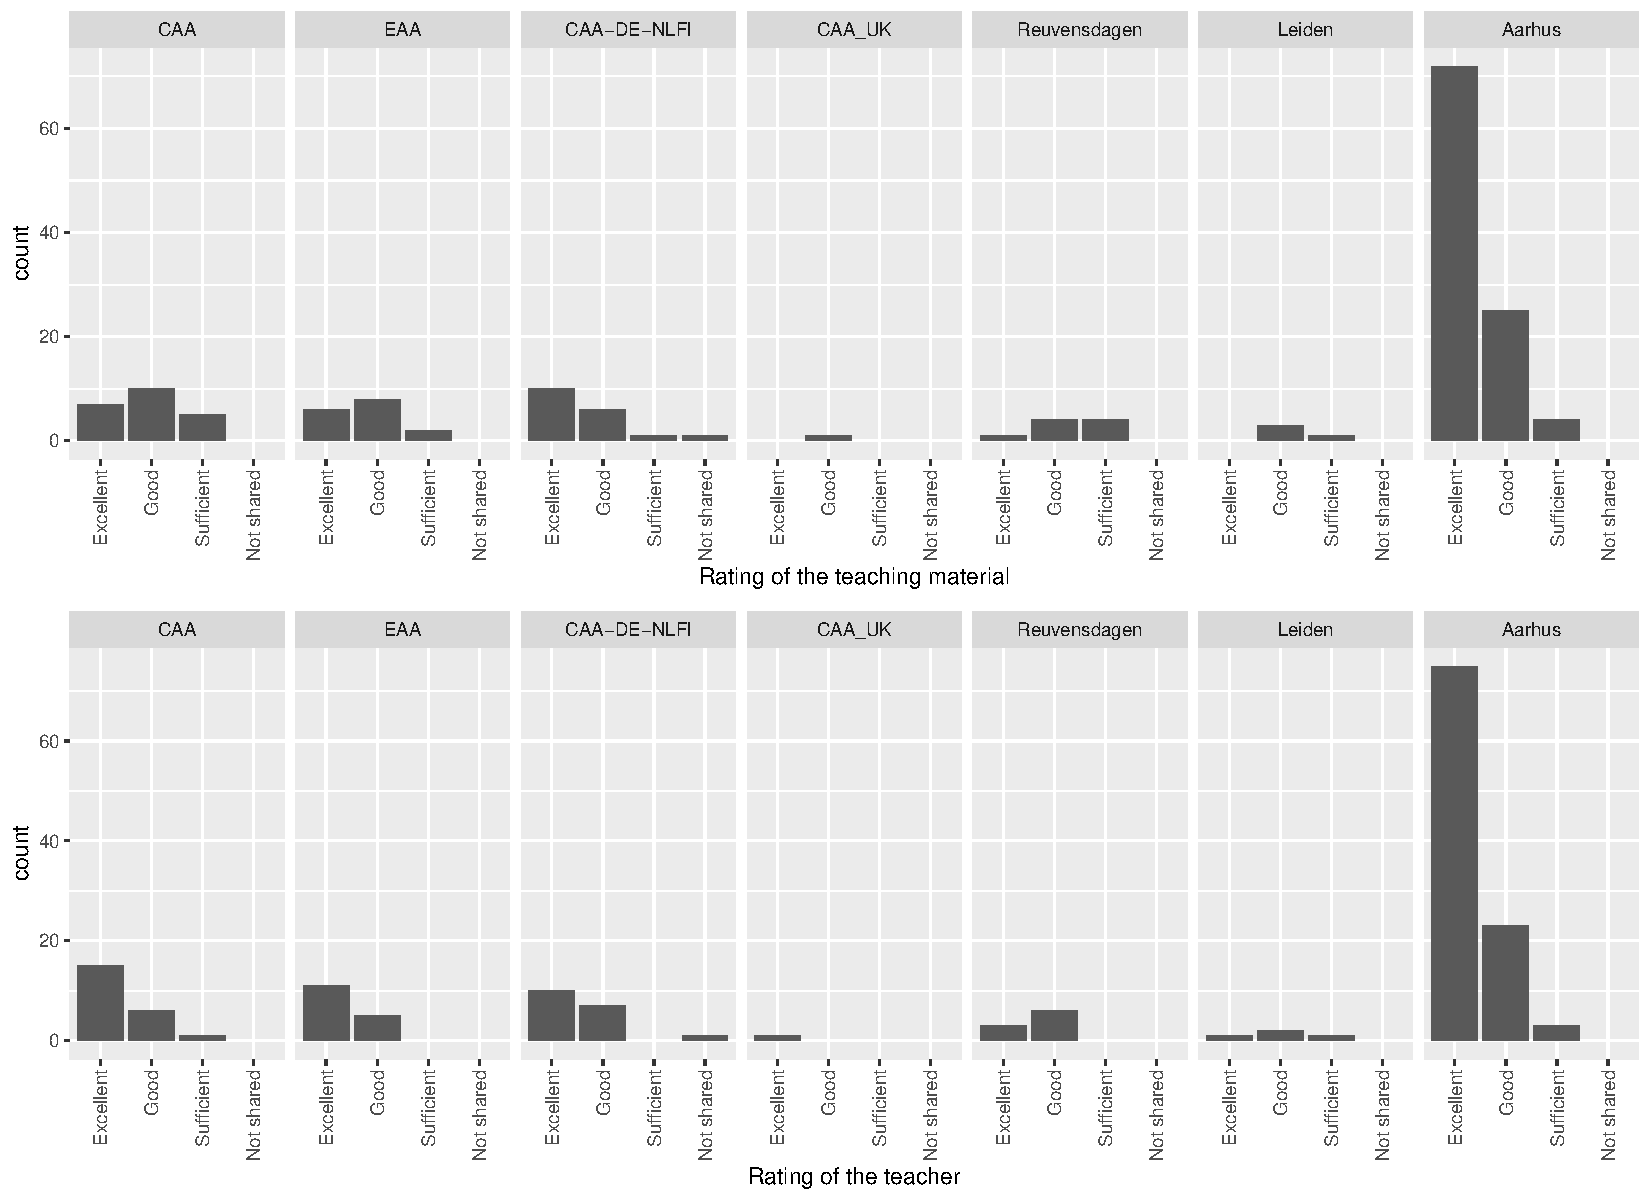
\includegraphics[height=0.5\textheight]{paper_files/figure-latex/rating-teaching-1} 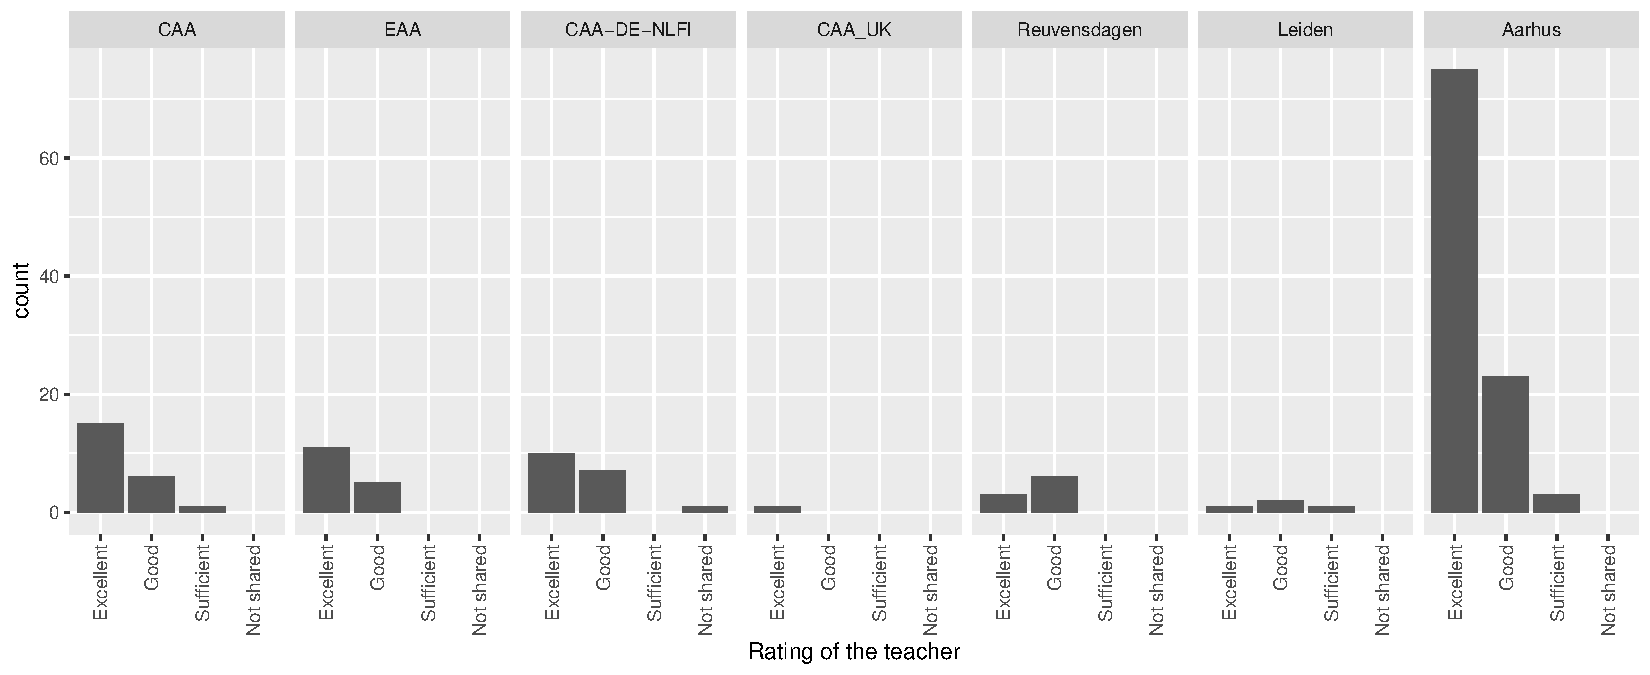
\includegraphics[height=0.5\textheight]{paper_files/figure-latex/rating-teaching-2} \caption{Respondents rating of the teaching material in general faceted for each event.}\label{fig:rating-teaching}
\end{figure}

Two more open questions were asked to the respondents. The first was aimed at getting positive feedback and the other was aimed at getting feedback to improve the tutorials.

The respondents generally liked the interactive step-by-step way of going through the tutorials, but also valued the interaction with the teachers very much. The easy and intuitive introduction into ABM and NetLOGO were also mentioned quite often. This was also observed during the workshops by us, most participants were working in the own pace and did not need much help. From a didactic point of view, the self-paced going through the tutorials is very efficient for teachers.

We also received feedback on possible improvements. For the first workshops we mostly received feedback on the number of bugs. During the CAA-conference in Amsterdam we did the first test of the tutorials and we also instructed the participants that this was work in progress. The number of references to bugs reduced to zero by the end and people started providing other feedback, for example the wish to see more examples or expanding the tutorials more. Some wanted more cooperation, which is possible, but for some online events harder, although we provided break-out rooms. It is also interesting to note that more and more people did not see any room for improvement.

The majority of the respondents that wanted to apply ABM in the future for research (144 of the 164 that answered this question, see Figure \ref{fig:future-abm}). Some of the respondents were already using ABM. A large group was not sure yet in how to apply ABM and wanted to read more on the subject or play a bit with the possibilities. Many respondents also shared the context in which they were thinking to apply ABM to. Various were thinking about movement of people or goods over land or water, sometimes in relation to trade or other distribution mechanisms. Others thought of demography, social networks, migration or settlement distributions patterns. The natural environment and the interaction with humans in the past was also mentioned by some, and often in relation to GIS or how to replace GIS with ABM. The archaeological periods that the participants were interested in were very diverse ranging from the paleolithic to the medieval period.

\begin{figure}
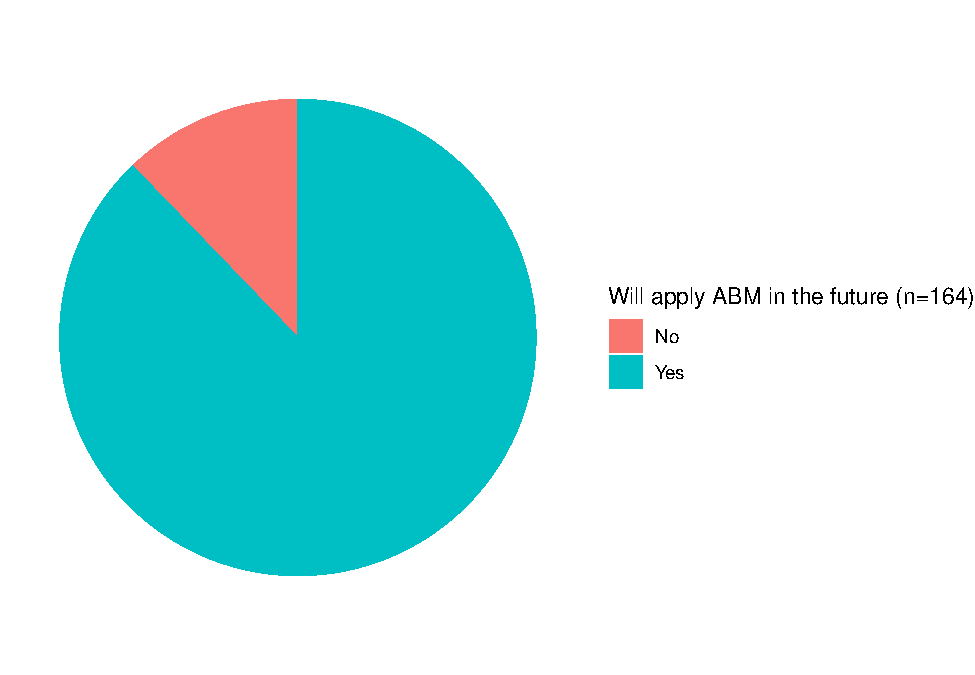
\includegraphics[height=0.5\textheight]{paper_files/figure-latex/future-abm-1} \caption{The respondents reaction to the question if they thing that they will apply ABM in the future.}\label{fig:future-abm}
\end{figure}

\hypertarget{final-tutorials}{%
\subsection{Final tutorials}\label{final-tutorials}}

\hypertarget{dissemination-of-tutorials}{%
\subsection{Dissemination of tutorials}\label{dissemination-of-tutorials}}

Website

Github

\hypertarget{conclusion}{%
\section{Conclusion}\label{conclusion}}

Lessons learned

Future aspects

\hypertarget{acknowledgements}{%
\section{Acknowledgements}\label{acknowledgements}}

We would like to thank the student groups at Saxion University of Applied Sciences that worked with us:

\begin{itemize}
\item
  September 2022-February 2023: Dany Dragoi, Liam van den Bosch, Marko Stojkovic, Max van Duinen, Nora van den Engel, Roan Man, Stefan Oostingh and their tutor: Mark Spanjer.
\item
  February 2022-July 2023: Alice Overgaauw, Johan Broersma, Mandy Hazenberg, Paulina Fulneczek, Ties Heesink and their tutor: Jan Willem Huson.
\item
  September 2023-February 2024: Arnfinn Sijbrant, Eva Baan, Jip Mulder, Robert Aalpoel, Sem Lucas, Sterre Regts and their tutor: Jan Willem Huson.
\end{itemize}

We had help from many people during the various workshops and we would like to thank them for their help (in alphabetical order of their first name): Adéla Sobotkova, Alice Overgaauw, Eduardo Herrera Malatesta, Jens Emil Bødstrup Christoffersen, Johan Broersma, Magnus Lindholm Nielsen, Mandy Hazenberg, María Coto Sarmiento, Paulina Fulneczek, Petra Hermankova, Ties Heesink. We also want to thank all the participants of our workshops.

\hypertarget{references}{%
\section*{References}\label{references}}
\addcontentsline{toc}{section}{References}

\hypertarget{refs}{}
\begin{CSLReferences}{1}{0}
\leavevmode\vadjust pre{\hypertarget{ref-grolemund2011}{}}%
Grolemund, G and Wickham, H. 2011 \href{https://www.jstatsoft.org/v40/i03/}{Dates and times made easy with lubridate}. \emph{Journal of Statistical Software} 40(3): 125.

\leavevmode\vadjust pre{\hypertarget{ref-rcoreteam2023}{}}%
R Core Team. 2023 \emph{\href{https://www.R-project.org/}{R: A language and environment for statistical computing}}.

\leavevmode\vadjust pre{\hypertarget{ref-romanowska2021}{}}%
Romanowska, I, Wren, CD and Crabtree, SA. 2021. \emph{\href{https://www.sfipress.org/books/agent-based-modeling-archaeology}{Agent-based modeling for archaeology: Simulating the complexity of societies}}. Santa Fe: Santa Fe Institute Press.

\leavevmode\vadjust pre{\hypertarget{ref-scherjon2019}{}}%
Scherjon, F, Romanowska, I and Lambers, K. 2019 Digitally Teaching Digital Skills: Lessons Drawn from a Small Private Online Course (SPOC) on {`}Modelling and Simulation in Archaeology{'} at Leiden University. \emph{Journal of Computer Applications in Archaeology} 2(1): 7988. DOI: https://doi.org/\href{https://doi.org/10.5334/jcaa.26}{10.5334/jcaa.26}.

\leavevmode\vadjust pre{\hypertarget{ref-wickham2016}{}}%
Wickham, H. 2016. \emph{\href{http://ggplot2.org}{ggplot2: Elegant graphics for data analysis}}. Springer-Verlag New York.

\leavevmode\vadjust pre{\hypertarget{ref-wickham2023b}{}}%
Wickham, H. 2023a \emph{\href{https://forcats.tidyverse.org/}{Forcats: Tools for working with categorical variables (factors)}}.

\leavevmode\vadjust pre{\hypertarget{ref-wickham2023c}{}}%
Wickham, H. 2023b \emph{\href{https://stringr.tidyverse.org}{Stringr: Simple, consistent wrappers for common string operations}}.

\leavevmode\vadjust pre{\hypertarget{ref-wickham2023a}{}}%
Wickham, H, François, R, Henry, L, Müller, K and Vaughan, D. 2023 \emph{\href{https://dplyr.tidyverse.org}{Dplyr: A grammar of data manipulation}}.

\leavevmode\vadjust pre{\hypertarget{ref-wickham2023}{}}%
Wickham, H, Vaughan, D and Girlich, M. 2023 \emph{\href{https://tidyr.tidyverse.org}{Tidyr: Tidy messy data}}.

\end{CSLReferences}

\end{document}
